\documentclass[12pt]{report}

\usepackage[top=1.2in, bottom=1.2in, left=1.4in, right=1.2in]{geometry}
\usepackage{graphicx}

\usepackage[T1]{fontenc}

\usepackage[francais]{babel}

\usepackage{fontspec}
\setmainfont{Droid Serif}
\setmonofont{Inconsolata}

\usepackage{url}
\usepackage{hyperref}
\usepackage{fancyhdr}
\pagestyle{fancy}

\usepackage{minted}

\linespread{1.3}

\definecolor{gray}{RGB}{155,155,155}
\definecolor{toogyblue}{RGB}{87,102,181}

\usepackage{indentfirst}

\newminted{ocaml}{bgcolor=gray!25,
                  fontsize=\normalsize,
                  mathescape,
                  linenos,
                  frame=lines,
                  framerule=0.3pt
                 }

\usepackage{titlesec, blindtext}
\definecolor{gray75}{gray}{0.75}
\newcommand{\hsp}{\hspace{20pt}}
\titleformat{\chapter}[hang]{\Huge\bfseries}{\thechapter\hsp\textcolor{gray75}{|}\hsp}{0pt}{\Huge\bfseries}

\fancyhf{}
\rhead{\textbf{\thepage}}
\lhead{\leftmark}
\rfoot{\leftmark}
\lfoot{\textbf{\thepage}}
\renewcommand{\headrulewidth}{0.4pt}
\renewcommand{\footrulewidth}{0.4pt}

\setcounter{tocdepth}{1}


\title{
\includegraphics[scale=0.55]{chapters/Pictures/kibi.png}}


\author{Mathieu `RustyCrowbar' Corre \\
        Thibaud `zehir' Michaud \\
        Valentin `toogy' Iovene \\
        Pierre `Grimpow' Gorjux
      }

\date{11 décembre 2013}

\begin{document}

\maketitle

\tableofcontents

\chapter*{Introduction}

This document will present the current state of our project, KiBiOCR, as part of
EPITA's syllabus. KiBiOCR's name speaks for itself. It is an OCR (Optical
Character Recognition) program. Its goal is then to recognize characters in a
given image.\\

You will see that our project is breaked up in 5 very distinct parts:

\begin{itemize}
    \item{Lenna}: preprocessing part of the program. Lenna modifies user's input
        image to help other parts of the program to do their job.
    \item{Freddy}: `he' is in charge of the segmentation part, which is
        identifying images, paragraphs, words and characters positions.
    \item{Anna}: this is our artificial neural network (ANN). `She' identifies
        characters segmented by Freddy.
    \item{\emph{(Le petit)} Robert}: this is our dictionary. `He' detects the
        document language and errors made by Anna/Freddy in the identification
        process and then try to find the nearest words.
    \item{Guy}: our user interface. This is the way our program and the user
        will be able to interact.
\end{itemize}

We gave surnames to the parts of our program because we like private jokes but
mainly because shortnames are really convenient when we talk about our project.

% \chapter{The team}
% 
% \section{Valentin `toogy' Iovene}
% 
% \begin{wrapfigure}{l}{0.1\textwidth}
%     \vspace{-1cm}
%     \begin{center}
%         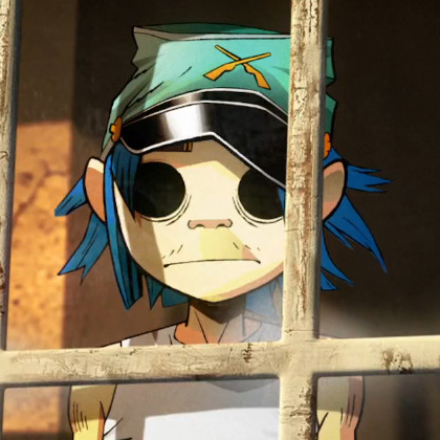
\includegraphics[width=0.1\textwidth]{images/toogy.png}
%     \end{center}
%     \vspace{-1cm}
% \end{wrapfigure}

\chapter{Lenna - \emph{Pré-traitement}}
Avant d'essayer de détecter les paragraphes, les lignes ainsi que les caractères dans l'image, et de reconnaître les caractères, il faut "nettoyer" l'image. Dans ce chapitre nous allons décrire différents algorithmes que nous avons implémentés dans ce but.\\

\section{Binarisation}
C'est le premier algorithme que nous avons écrit parce qu'il est simple, essentiel et c'est un bon point de départ pour se familiariser avec la bibliothèque et ses fonctions de base. Nous avons d'abord implémenté la méthode la plus naïve : calculer la moyenne des composantes RGB de chaque pixel pour avoir sa luminosité, et appliquer un seuil. Tout pixel dont la luminosité est en dessous de 127 est considéré comme blanc et les autres comme noir. Evidemment, ce ne fut pas notre algorithme définitif.\\

Nous aurions pu l'améliorer en prenant comme seuil la luminosité moyenne des pixels, cependant cela n'aurais pas été beaucoup mieux. Nous avons plutot décidé de rechercher un meilleur algorithme, et avons décidé que la méthode d'Otsu était la plus adaptée à notre cas. De plus cet algorithme est relativement simple à impémenter. La principe de la méthode d'Otsu est de trouver le seuil idéal pour l'algorithme décrit précedemment. Le seui idéal est défini comme étant celui qui minimise la variance entre les deux classes formées par ce seuil. Il faut donc essayer chaque seuil possible et calculer à chaque fois la variance de chaque classe. Heureusement une petite astuce mathématique nous permet de réduire de façon significative la complexité de cet algorithme en maximisant la variance inter-classe au lieu de minimiser la variance intra-classe.\\

\section{Réduction du bruit}

Nous avons éssayé deux méthodes pour réduire le bruit dans l'image : le flou gaussien et le filtre médian. Nous avons été insatisfait des deux car les lettres étaient moins lisible après le filtre. Pour corriger ça, nous avons réduit le nombre de pixel voisins pris en compte dans le filtre median : pour chaque pixel, nous prenons le pixel median parmi le pixel lui même et ses quatre voisins immédiats.\\

\section{Rotation}

\subsection{Algorithme de base}

Il est très difficile voir impossible (ou du moins contre-productif) de
détecter des zones de textes, caractères, mots dans une image si cette image
n'est pas droite. C'est pourquoi il est nécessaire, au cours de l'étape de
pré-traitement \emph{pre-processing}, de roter l'image fournie par l'utilisateur
afin qu'elle soit bien adaptée aux étapes de segmentation et d'identification
des caractères. \\

\subsubsection{Implémentation naive}

Une implémentation naive de la rotation serait l'algorithme suivant. C'est
celui que nous utilisions à la première soutenance mais qui posait quelques
soucis. \\

\begin{itemize}
  \item{Input}
    \begin{itemize}
      \item Image de base
      \item Angle de rotation $\theta$
    \end{itemize}
  \item{Output}
    \begin{itemize}
      \item Image rotée
    \end{itemize}
\end{itemize}

\begin{enumerate}

  \item Soit $(w, h)$ les dimensions de l'image de base. Calculer les dimensions
    $(nw, nh)$ de l'image après qu'une rotation d'angle $\theta$ soit appliquée
    sur l'image de base. Visuellement, les dimensions de l'image de base et de
    l'image rotée sont liées par une simple relation trigonométrique.
  \begin{center}
    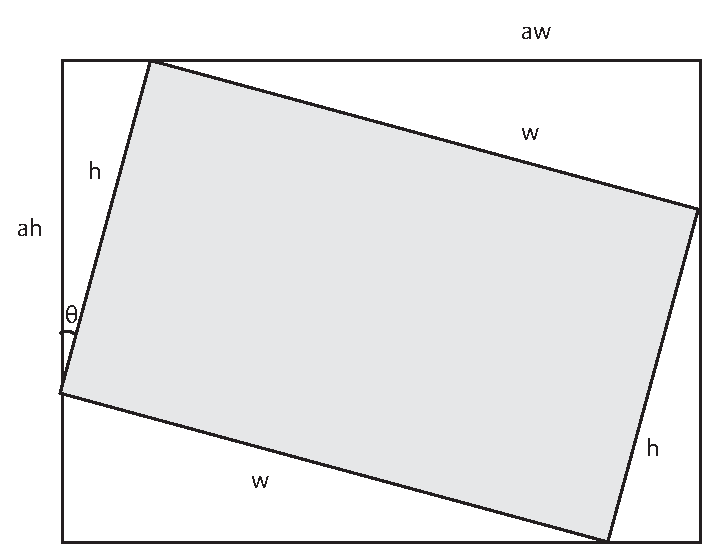
\includegraphics[scale=0.75]{chapters/Pictures/toogy/rotation-new-size.eps}
  \end{center}

  \item Créer une nouvelle image de dimensions $(nw, nh)$ remplie de blanc.

  \item Pour chaque pixel de la nouvelle image, matérialisé par ses coordonnées
    $(x,y)$ dans l'image rotée, calculer ses anciennes coordonnées $(x',y')$
    dans l'image de base. Pour ce faire, on a la relation: \\ 
    $$\begin{pmatrix}x'\\y'\end{pmatrix} =
      \begin{pmatrix}
        \cos\theta & -\sin\theta \\
        \sin\theta & \cos\theta
      \end{pmatrix}
    \begin{pmatrix}
      x \\
      y
    \end{pmatrix}$$

  \item Arrondir ces nouvelles coordonnées et donner aux pixel $(x,y)$ de la
    nouvelle image la couleur du pixel $(x',y')$ de l'image de base. Renvoyer
    l'image.

\end{enumerate}

Cependant, cet algorithme déforme légèrement l'image. Ici, il s'agit de texte et
cette petite déformation réduit énormément sa lisibilité; pour l'homme comme
pour la machine. Il s'agit donc d'être plus intelligent.

\subsubsection{Interpolation Bilinéaire}

\paragraph{Interpolation mathématique\\}

En mathématiques, une interpolation consiste à se servir de données déjà
existante pour approximer des données qui nous manquent. \\

Une interpolation peut se faire de plusieurs façons; plus ou moins précises.
Bien sûr, qui dit plus de précision dit plus de temps de calcul.

\paragraph{Interpolation bilinéaire appliquée à la rotation\\}

Ici, il s'agit de se servir des pixels de notre image de base (nos données) pour
déterminer les pixels de notre nouvelle image (les données que nous allons
interpoler). \\

Plusieurs algorithmes d'interpolation existent :
\begin{itemize}
  \item{Nearest-neighbor Interpolation} : le plus simple, il consiste à faire
    la moyenne des composantes $(r,g,b)$ des pixels voisins de notre pixel
    $(x',y')$. C'est le plus rapide.
  \item{Bilinear Interpolation} : un peu plus complexe, il s'agit ici de faire
    deux interpolations linéaires : une entre les deux pixels au dessus de
    $(x',y')$ et une autre entre les deux pixels en dessous de $(x',y')$ (les
    valeurs $x'$ et $y'$ n'étant évidemment pas approximées mais bien située
    entre les entiers de l'arrondi supérieure et de l'arrondi inférieur des
    coordonnées).
    \begin{center}
      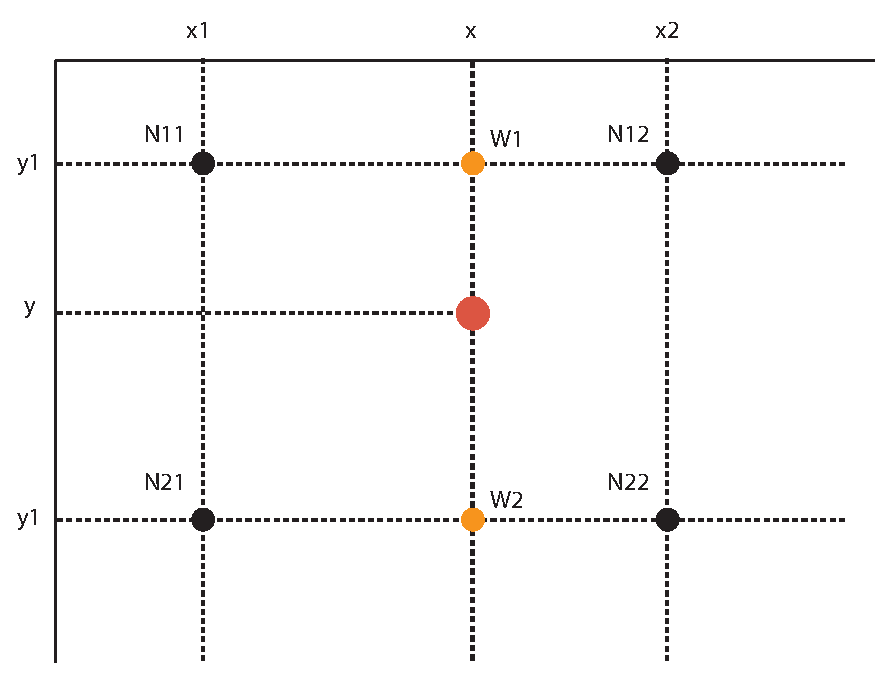
\includegraphics[scale=0.75]{chapters/Pictures/toogy/bilinear.eps}
    \end{center}
    On a alors : \\
    $$W_{1} = \frac{x_{2} - x}{x_{2} - x_{1}} N_{11}
    + \frac{x - x_{1}}{x_{2} - x_{1}} N_{21}$$ \\
    $$\text{et } W_{2} = \frac{x_{2} - x}{x_{2} - x_{1}} N_{12}
    + \frac{x - x_{1}}{x_{2} - x_{1}} N_{22}$$ \\
    Les nouvelles composantes du pixel peuvent alors être calculée via la
    formule \\
    $$R = \frac{y_{2} - y}{y_{2} - y_{1}} W_{1}
    + \frac{y - y_{1}}{y_{2} - y_{1}} W_{2} \text{ \emph{(cas de la
    composante rouge du pixel)}}$$
  \item{Bicubic Interpolation} : plus longue de part son temps de calcul, c'est
    le même principle que pour l'interpolatian bicubique sauf que 8 pixels sont
    étudiés au lieu de 4. Elle donne des résultats plus esthétiques qui ne sont
    pas vraiment utiles dans notre cas.
\end{itemize}

\paragraph{Résultat}

\begin{figure}
  \centering
  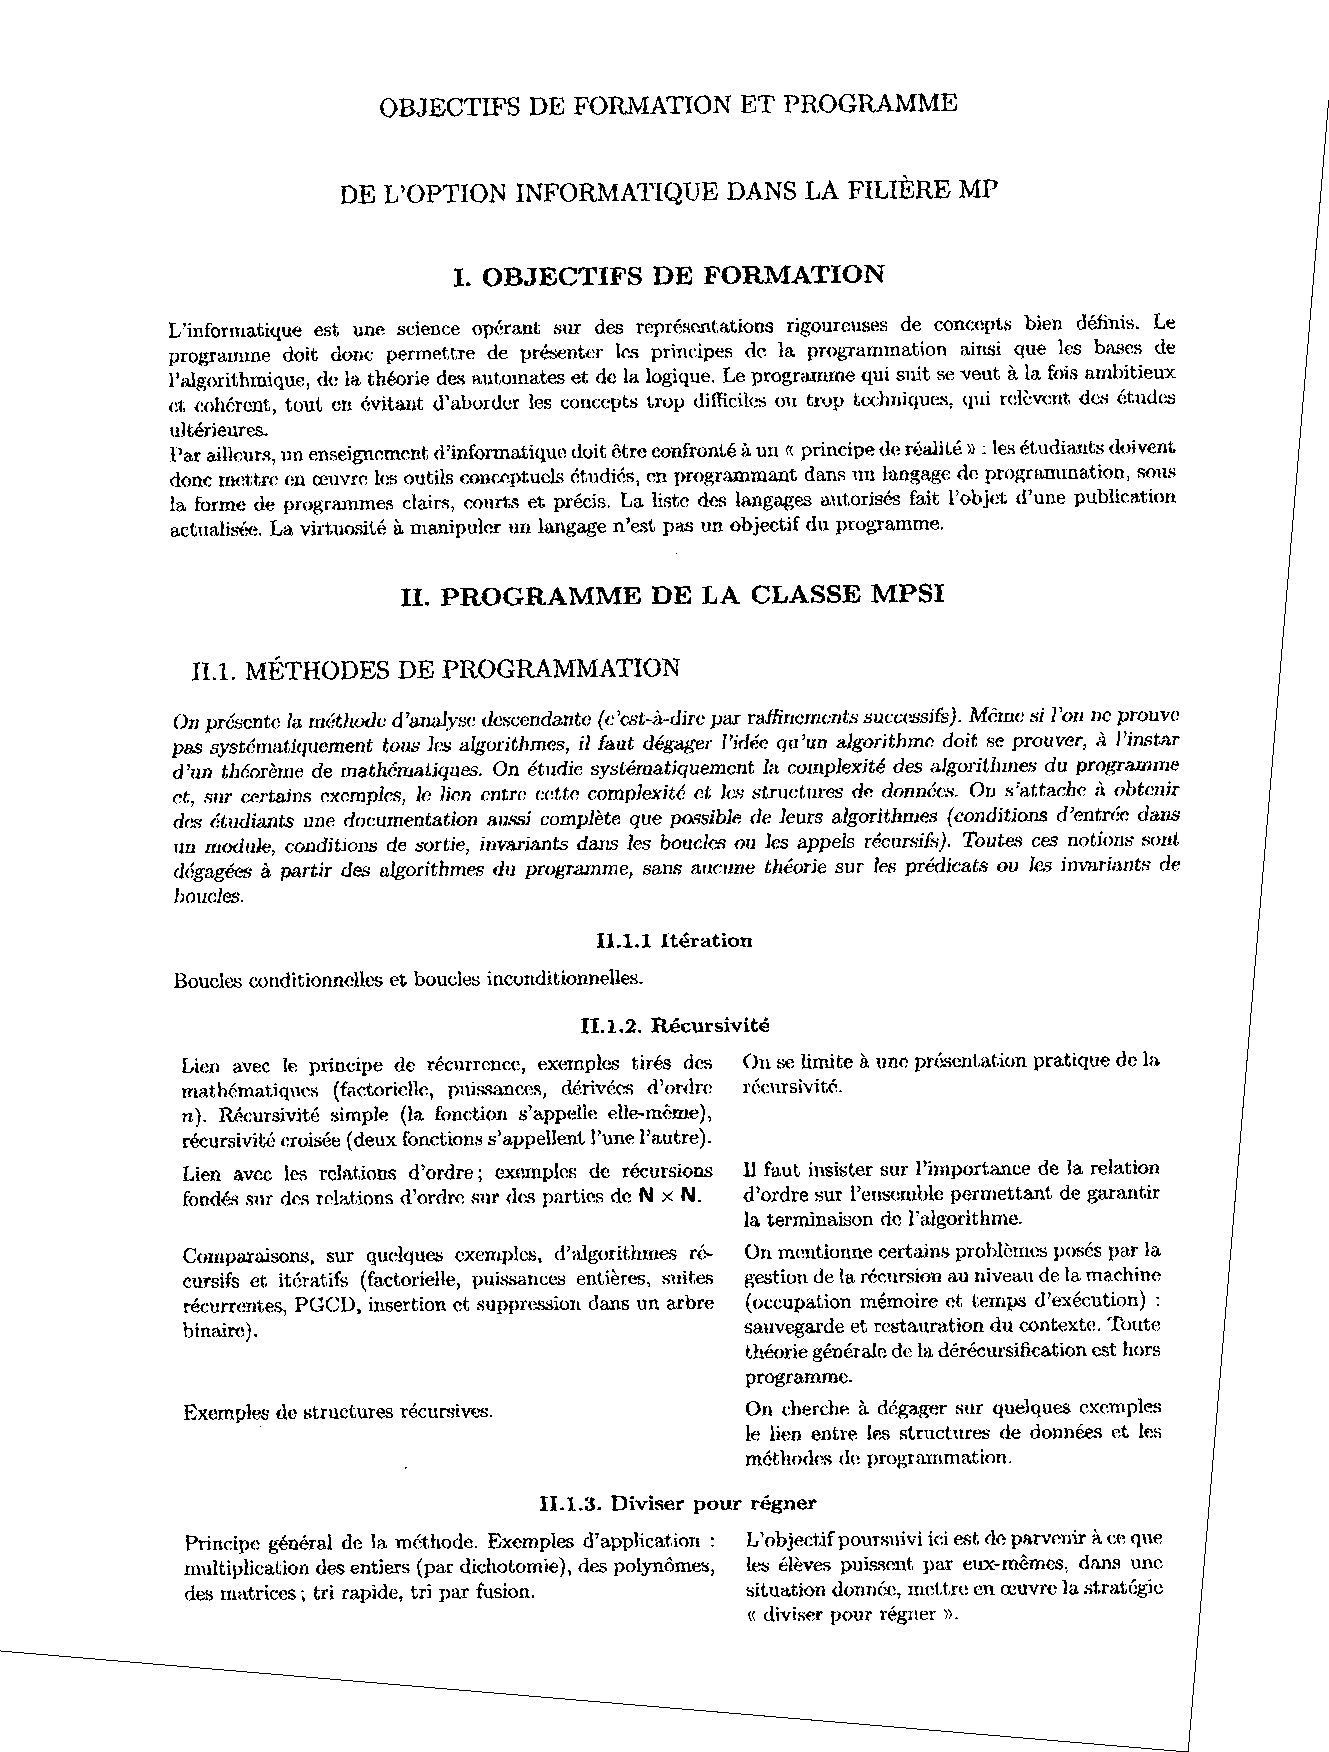
\includegraphics[scale=0.5]{chapters/Pictures/toogy/rotation.eps}
\end{figure}

\subsection{Détection de l'angle}

\subsubsection{Transformée de Hough}

La transformée de Hough est une méthode générale pour trouver des lignes et des ellipses dans une image. Elle est souvent utilisée car une fois le principe mathématique compris, elle est simple à implémenter, donne de bons résultats et à une complexité assez faible par rapport, par exemple, à la transformée de Fourier. Nous n'avons besoin que du cas le plus simple de l'algorithme qui consiste à trouver les lignes dans une image binarisée.

La transformée de Hough se base sur une représentation très particulière des droites du plan : plutot que deux les représenter avec les deux paramètres usuels $a$ et $b$ dans l'équation $y = ax + b$, une droite est décrite comme un couple $(r, \theta)$ où $r$ est la distance de la ligne à l'origine et $\theta$ est l'angle de cette distance par rapport à l'abscisse.

  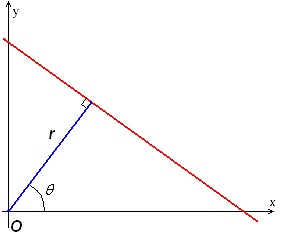
\includegraphics[scale=0.5]{chapters/Pictures/hough1.jpg}\\
En quoi cette représentation est-elle utile? Cela vient du fait que, étant donné un point de coordonnées $(x, y)$ et l'angle $\theta$ de la droite passant par ce point, il est facile d'exprimer la distance $r$ entre la ligne et l'origine. L'équation est la suivante :\\
$r = x\cos\theta + y\sin\theta$\\
Donc pour un point de coordonnées $(x, y)$ on peut tracer le graphe de $r$ en fonction de $\theta$. Il est facile de deviner d'après l'équation que ce graphe sera une sinusoïde. Cette sinusoïde représente l'ensemble des droites passant par ce point. Si nous stockons ce graphe dans un accumulateur, et ajoutons dans cet accumulateur la sinusoïde correspondant à tous les autres points, on obtient un graphe tableau dans lequel la valeur la plus grande représentera les coordonnées de la droite (dans l'espace de Hough) passant par le plus de points possible.

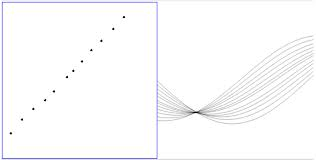
\includegraphics[scale=0.7]{chapters/Pictures/hough2.jpg}\\
\subsubsection{Plus de pré-traitement}

Il y'a encore un problème à régler avant de pouvoir appliquer la transformée de Hough à notre image scannée : Une ligne de texte n'apparait pas comme une ligne droite. Nous avons essayé d'appliquer directement à une image binarisée, mais la plupart du temps il trouvait ou bien la diagonale de l'image, ou bien une reliure particulièrement visible. Après quelques recherches, nous avons trouvé une solution : on détecte tout d'abord les blocs de pixels noirs connexes, qui ne sont pas toujours mais très souvent des caractères, et on les remplaces par leur point centrale. L'utilité est triple : rendre plus apparentes (du point de vue de la transformée de Hough) les lignes de texte, réduire considérablement la complexité de l'algorithme et reduire l'importance des gros blocs de pixels comme les tâches ou les reliures. Voici un exemple de sortie :

\begin{figure}[h!]\
    \centering
    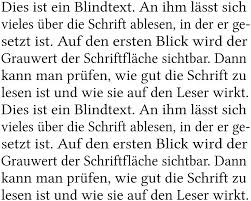
\includegraphics[scale=1]{chapters/Pictures/hough3.jpg}
    \caption{input image}
\end{figure}
\begin{figure}[h!]\
    \centering
    
\includegraphics[scale=1]{chapters/Pictures/hough4.jpg}
    \caption{center of each block}
\end{figure}
\begin{figure}[h!]\
    \centering
    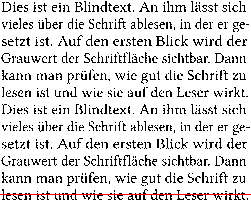
\includegraphics[scale=1]{chapters/Pictures/hough5.png}
    \caption{line found by the Hough transform}
\end{figure}


\chapter{Freddy -- \emph{Segmentation}}

Freddy is our segmentation module. It uses OCSFML.
To detect lines as today, we first assume that all the previous preprocessing steps were done perfectly, which means no artefacts, good rotation, binarization... For now, we can only get text, in one column, and no images. We will work on those situations, and Freddy will be working as expected on time.

Freddy est notre module de segmentation, il utilise OCSFML.

\section{L'ancienne méthode, ses points faibles}

Au moment de la première soutenance, nous utilisions un algorithme très simple, et moyennement efficace: nous faisions un histogramme horizontal, un tableau de taille la hauteur en pixels de l´image. Nous le remplissions avec le nombre de pixels noirs à la ligne correspondante. Cette opération nous permettait de savoir à quel moment une nouvelle ligne ou un nouveau paragraphe apparaissent.\\
Une fois ce découpage effectué, il nous suffisait de répéter cette opération horizontalement sur chacune des lignes repérées, afin de détecter les mots et caractères composant chacune des lignes.\\
Cependant, nous avons été confrontés à plusieurs problèmes, qui nous ont amenés à chercher une autre méthode plus performante, que nous verrons en détail dans la prochaine section. En effet, avec cette méthode, les caractères avaient tendance à être coupés, ou bien collés à d´autres. Il en était de même pour les lignes, qui avaient tendance à fusionner. Cette technique nécessitait également d´avoir une image sortie du prétraitement parfaite, la moindre impureté ou la moindre ligne, image ruinant totalement le résultat de l´algorithme.

\section{Le RLSA}

Pour détecter les paragraphes, lignes, mots ou les caractères, nous utilisons donc maintenant l'algorithme Run Lenght Smooth Algorithm (RLSA) modifié par nos soins, pour couvrir au mieux nos besoins. Le principe est simple: on regarde horizontalement et verticalement quels sont les pixels noirs adjacents, c´est à dire quels sont les pixels noirs séparés de moins de n pixels noirs. Il en résultera donc deux matrices de bouléens aux dimensions de l´image. Dans ces matrices représentant la couleur noire ou blanche des pixels de l´image, nous aurons changé tous les pixels blancs entre deux pixels noirs adjacents. Les images représentées par ces matrices ressemblent à l´image d´entrée, mais comme si l´encre avait bavée horizontalement ou verticalement.

\subsection{Optimisations}

\begin{center}
\end{center}

\begin{center}
\end{center}

\section{Line and character detection}

\subsection{Making horizontal/vertical histogram}

To detect lines, we need to make histograms, containing the number of black pixels in every line/column of line of pixel of the provided image.We put everything in lists.

\subsection{Delimit lines/characters}

When the number of black pixel changes a lot, we decide to create or to end a line/to create or end a character. We put it in lists.

\subsection{Delimit lines/characters}

When the number of black pixel changes a lot, we decide to create or to end a line/to create or end a character. We put it in lists


\chapter{Anna -- \emph{Identification}}

After we have preprocessed the image and found the paragraphs, lines and characters in the document, we need to recognize these characters. To do this, we use a machine learning technique called a feed-forward neural network. In this chapter, we will describe in detail the result of our researches on the subject.

\section{Machine learning}

Machine learning is a field of research in which we try to design "agents" able
to improve their performance on a given task with experience. In the case of an
OCR software, the agent's task will be to classify images of characters, and the
experience will consist of feeding the agent with many examples. The examples
will be pairs of the form (image of the character, corresponding character).

\section{Univariate linear regression}

Lets look at a simpler problem: we have examples of the form $(x, y)$ where $x$
and $y$ are numbers, and our goal is to find a straight line to fit the
examples.\\

\begin{center}
\end{center}

The line will be of the form $h_w(x) = w_1x + w_0$. In order to determine the
most fitting line, we first need to define an error function. The sum of the
squared error appears to have nice properties (as being positive and
differentiable). This error function is expressed as follows:
$Loss(h_w) = \sum\limits_{j=1}^{N}(y_j - h_w(x_j))^{2}$. Now we need to minimize
this. To understand how we do this, it helps to visualize the graph ofthe Loss
in function of $w$.\\

Now imagine we start at a random point on this graph (i.e., we start with a
random line). To get to the minimum of the function, we only need to follow the
slope downward. Mathematically, this translates as substracting the gradient of
the Loss function from the current point, since the gradient points toward the
steepest slope upward. We usually multiply the gradient by a constant called the
learning rate, noted $\alpha$, to regulate the size of the steps. A slow
learning rate means converging slowly but a large learning rate might lead to
stepping over the minimum. The update rule is then:\\

$w_i \leftarrow w_i - \alpha \frac{\partial}{\partial w_i} Loss(w)$\\

We won't compute the derivative right now as we don't need it.

\section{Multivariate linear regression}

The extension to a multivariate problem is pretty straight forward. Lets denote
by $\textbf{x} = (x_0, x_1, ..., x_n)$ the input vector. The estimation function
then becomes $h_w(\textbf{x}) = w_nx_n + ... + w_1x_1 + w_0x_0$.

\section{Logistic regression}

What we want is a classification algorithm. We only need to slightly modify the
previous algorithm to make it a binary classifier: we keep the estimation
function $h_w(x)$, but we then feed the result to another function whose output
is in $[0;1]$. One such function is the step function, which worth 0 if $h_w(x)$
is negative and 1 otherwise. But this function is not differentiable, and we
will see later that it is a problem. So we usually prefer the logistic function,
or sigmoid function:\\

\begin{center}
\end{center}

Its equation is $g(x) = \frac{1}{1 + e^{-x}}$, and its derivative is
$g(x)(1 - g(x))$. Applying the same algorithm as for the multivariate linear
regression, the update rule becomes:\\

$w_i \leftarrow w_i + \alpha (y - h_w(\textbf{x}))
h_w(\textbf{x})(1 - h_w(\textbf{x}))x_i$\\

There is no need here to explain the derivation of the Loss function.

\section{Perceptron}

The logistic regression function will be the elementary brick for our neural
network. It is what we will call a neuron, since it is very close to the real
principle of biological neuron. Now lets complexify the problem a little bit: we
need to classify the input data between more than two possible outcomes. Let's
say for example that we need three possible outcomes. We only need to connect
the input to three different logistic regression units. This will produce an
output vector instead of a single value, and ideally this vector will converge
toward something like (1, 0, 0), (0, 1, 0) or (0, 0, 1), each time representing
one of the three possible cassifications. This is called a single-layer
feed-forward neural network, or perceptron.\\

\begin{center}
\end{center}

\section{multi-layer feed-forward neural network}

A feed-forward neural network is a perceptron, whose output will be the input of
another perceptron, etc. until it reaches the output layer. Every layer that is
not the input layer or the output layer is called a hidden layer. The big
advantage of a multi-layer feed-forward neural network over a perceptron is that
it can potentially compute any continuous function with only one hidden layer
and with the right number of neurons in each layer, according to the universal
approximation theorem.\\

\begin{center}
\end{center}

What changes between the perceptron and the multi-layer feed-forward neural
network is the derivative of the loss function. Once again, there is no need to
enter into the details of the maths behind the derivation, but the only thing we
need to know when implementing the neural network is that the derivative of the
parameters in one layer depends on the derivative of the parameters of the next
layer. Therefore we need to compute the derivative in the output layer, then the
hidden layer, hence the term "backpropagation".

\section{Optimizations}

The only optimization we implemented at this point is the momentum. In the
gradient descent process, we can consider that the current point has some
inertia by adding a certain percentage of the gradient of the last iteration in
the update rule. There are two purposes to this: converging faster, and avoiding
local minimum.


\chapter{Robert - \emph{Spell checking}}

Robert est un module capable de détecter le langage utilisé dans un texte donné, et éventuellement
 indiquer à l'utilisateur les différentes fautes que peut contenir ledit document en lui donnant une
sélection de mots considérés comme étant probables.  

\section{Génération des Dictionnaires}
Un dictionnaire est un fichier contenant un ensemble de mots, appartenant à une langue spécifique,
que l'on peut retrouver dans un texte.\\
Nous ne les avons pas généré, c'est un travail bien trop fastidieux, d'autant plus qu'il est aisé d'en
trouver sur Internet, sous la forme de fichier texte doté d'un mot par ligne ; Par exemple, un dictionnaire
anglais ne contient pas moins de 150 000 mots, et le dictionnaire français passe la barre des 700 000.
Seulement, si à chaque fois que l'on souhaitait vérifier l'existence d'un mot dans une langue donnée, il
faille parcourir les 700 000 lignes du fichier de manière séquentielle, le temps pris risque d'être énorme,
d'autant plus qu'un texte n'est généralement pas composé d'un seul mot, mais de plusieurs centaines, voir des
milliers. C'est pourquoi nous effectuons un prétraitement lors de l'ajout d'une langue à Robert : il s'agit
de la génération d'une structure de données au temps de recherche constant contenant l'ensemble des mots
appartenant à la langue donnée : La table de hashage, ou hashtable s'est donc imposée par défaut, grâce à
son temps de recherche constant, quelque soit la taille de l'ensemble qu'elle contient. \\
Ainsi, lors du chargement de Robert, OCaml va générer à partir des fichiers dictionnaires de chaque langue
reconnue des nouveaux dictionnaires (qui sont des hashtable)  reconnaissant la langue en RAM. \\
Un dernier soucis reste que la génération de ces dictionnaires nécéssitent obligatoirement une lecture
séquentielle de la hashtable, ainsi qu'un certain nombre de calculs quant à leur générations. \\Au final,
le chargement entier de la table de hash à partir du fichier texte ne prend pas moins de 1 seconde par langage.
Dans le doute, si jamais Robert devait être capable de gérer plusieurs dizaines de langages, le programme prendrait
pas moins de plusieurs dizains de secondes, rien qu'au chargement du module.

La solution a été trouvée grâce au module Marshall D'OCaml, qui permet de sérialiser un object en un tableau de bytes,
c'est à dire de copier sa représentation RAM dans un tableau de byte, et inversement. L'intérêt majeur est qu'il s'agit
d'une opération peu chère, qui permet de sauvegarder alors ce tableau dans un fichier binaire, pour le recharger
éventuellement plus tard. La génération du dictionnaire à partir du fichier source n'a alors à être réalisée qu'une
seule et unique fois par les développeurs, et Robert chargera et désérializera alors les dictionnaires à chaque fois
où KibiOCR sera appelé. Le gain apporté est assez conséquent, étant donné que l'on peut constater d'une ammélioration
de vitesse approchant les 1 000\%

\section{Détection d'un langage dans un texte donné}
L'algorithme de détection de langage actuellement utilisé est assez simple et redoutable d'efficacité :\\
Il analyse les X premiers mots (ou moins si le texte en fait moins) du texte qu'on lui donnera ; pour chaque langage, il contera alors le nombre de mots
reconnus. Une fois au les X mots traités, le langage retenu par la détection sera alors celui ayant le plus de termes reconnus.\\
\\
La constante X a été définie à 200, ce qui reste un nombre raisonnable du point de vue temps pris, tout en permettant de passer outre les
éventuelles erreurs que le texte peut comporter.\\
\section{Détection des termes incorrects}
La démarche utilisée est à peu près similaire ; robert va lire mot par mot l'ensemble du texte. A chaque fois qu'un mot n'existe pas dans le dictionnaire,
Robert va alors chercher quels mots pourraient correspondre. 
\section{Sélection des corrections possibles}
Généralement, quand un mot est incorrect, c'est que l'utilisateur l'ayant tapé l'a avant tout pensé phonétiquement, et a donc écrit correctement le mot,
phonétiquement parlant. Ainsi, "partez", qui est correct, peut devenir "parté", qui lui est incorrect.\\
Le système de correction orthographique de Robert a été pensé pour palier à cette déficience humaine, qui tend à empirer de nos jours...\\
C'est pourquoi nous avont implémenté en tout premier lieu l'algorithme phonétique Soundex, qui permet de générer une chaine phonétique à partir de n'importe
quel mot, à condition de connaître la langue auquel il appartient, étant donné que les prononciations varient sensiblement d'une langue à une autre, par exemple
entre le marseillais et le ch'ti.
L'algorithme se base sur le fait que ce qui permet d'identifier la prononciation phonétique d'un mot, ce ne sont pas les voyelles, mais au contraires les consonnes ;
Il va donc éliminer dans un premier temps toutes les voyelles du mot. Ensuite, les consonnes sont associées à un groupe donné, et remplacées par le chiffre correspondant :\\
\begin{itemize}
	\item 1 = B, P
	\item 2 = C, K, Q
	\item 3 = D, T
	\item 4 = L
	\item 5 = M, N
	\item 6 = R
	\item 7 = G, J
	\item 8 = X, Z
	\item 9 = F, V
\end{itemize}
Cette liste de groupes correspond à la pronciation français, il va de soi que pour l'anglais, elle varie: \\
\begin{itemize}
	\item 1 = B, F, P, V
	\item 2 = C, G, J, K, Q, S, X, Z
	\item 3 = D, T
	\item 4 = L
	\item 5 = M, N
	\item 6 = R
\end{itemize}
Ensuite, toutes les redondances de chiffres (par exemple P suivi de F donnera 11 en anglais, ce qui est une redondance) sont réduites à un seule chiffre,
et la chaîne de caractères ainsi obtenue est une chaîne phonétique Soundex.\\
Maintenant que l'on sait si deux mots donnés sont phonétiquement équivalents, il faut être capable de trouver l'ensemble des mots équivalents ; c'est 
pourquoi nous allons encore une fois passer par les merveilleuses table de hashage, afin de générer un dictionnaire phonétique.\\
Avant la mise en production, différents dictionnaires phonétiques sont générés en fonction des langues, qui à une chaîne soundex donnée, renvoient
 une liste contenant tous les mots équivalents. 
Seulement, il arrive que plusieurs dizaines de mots puissent être proposés, et afin d'éviter que l'utilisateur se perde (se noie) dans le flot de propositions,
il est impératif de trier l'ensemble, afin de sortir uniquement les X termes jugés les plus pertinants. Il est évident que si un mot fait 6 lettres, il est inutile
de proposer des choix de 42 lettres, les probabilités que l'utilisateur aie voulu taper le mot de 42 lettres étant malheureusement trop faibles.\\
C'est pourquoi un deuxième algorithme intervient alors, qui mesure la distance d'édition entre deux mots, c'est à dire qui mesure le nombre minimal d'opérations élémentaires
(déletion, ajout, remplacement) nécéssaires afin de transformer un mot A en un mot B. Cet algorithme est la "distance de Levenshtein".\\
La liste totale des éventuelles propositions est alors triée par ordre croissant en fonction de la distance de levenshtein entre chaque mot de la liste et le mot originel incorrect,
et seuls les X premiers termes de la liste sont alors retenus, X ayant été choisi par défaut comme étant 5.
Robert permet ainsi une proposition de correction orthographique puissante.
\begin{center}
	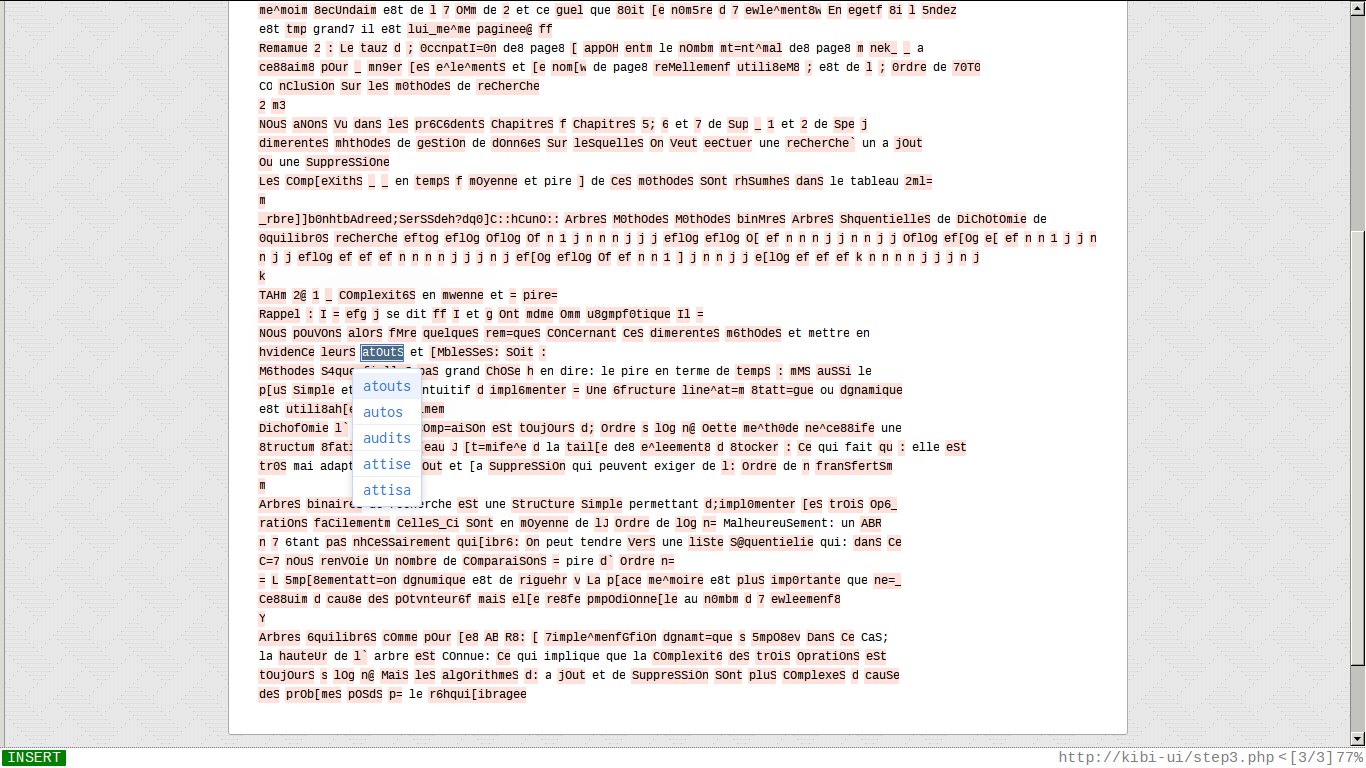
\includegraphics[scale=1]{Pictures/robert.png}
	\caption{Notre bon vieux Robert à l'action}
\end{center}


\chapter{Guy - \emph{Graphical User Interface}}

\section{A quick overview of Guy}

Guy is our GUI. It uses LablGTK and OCSFML, and will probably be using html to render the text output. It has several roles that we will describe right now. It is today composed of one window, to choose the file. It will be, for the second soutenance, composed of two or three more windows, to show the flow of the processing and the time taken by every main algorithm that we are using. 

\begin{center}
\end{center}

\section{A user-friendly interface}

\subsection{Helping the user to choose the image to process}

Guy has a built-in file browser, which is very intuitive, and easy to use, to select the file you want to use. Once the file has been selected, it's path will be displayed in an editable text box. However, the user can directly type in the provided text box the path of his desired file. Of course, it is still possible to use our program via the command-lines.

\subsection{Displaying the usefull informations}

We will display a miniature image of the image (assuming that it really is an image) that the user choosed.

\subsection{Showing the final result to the user}

Guy will be charged to show to the user the final work of our OCR. Indeed, we will present the image the user gave us, and the text we could detect, with the eventual orthograph corrections using Robert. It needs to be well organised, so that in case of a long document, the user could find where everything in the output text is located in his image, and vice-versa.

\section{Guy is the foreman}

One of the role of our GUI is to make every module work one after the other, calling them one after the other, with the right parameters. It will be possible to include one or several progress bars to inform the user of the flow of the processing.

 
\chapter{Website}

\section{Python}

\begin{center}
\end{center}

This year, we decided to switch from PHP to Python. We think that Python is a
stronger and more relevant language and we wanted to learn its syntax and its
specifics. So, here we are. \\

Plus, if we want to put our OCR online so that people can use it via a web
interface, it would me so much easier to do it with Python than with PHP. Python
can easily call other programs and execute commands on the server in a very
secure way. It is more complicated with PHP.

\section{Django}

\begin{center}
\end{center}

There is a very nice Python web framework out there on the web that is called
Django. Working with Django is quick: it is made for rapid development and for
perfectionists (we are).

\section{Nginx}

\begin{center}
\end{center}

We wanted to use something else than a basic Apache server so we decided to go
with Nginx, a quick, clean and easy to configure web server.

\section{Github}

\begin{center}
\end{center}

Our code is hosted on the now very famous website (and git server) GitHub. For
the moment, it is located in a private repository (for obvious reasons) but we
plan to go opensource once the last soutenance will be passed!


\chapter*{Conclusion}

Our project is moving forward very well. Our team is organized, we are all
working with passion and seriousness. We often schedule meetings and establish
task lists so that everyone is aware of what has to be done and can pick up
something he is interested in. \\

Some very tough tasks are waiting for us and we hope we will be able to show up
at the final with a fresh and working piece of art.

\end{document}


